\section{初等范畴论}

\subsection{范畴与函子}

\begin{definition}[范畴]
    \label {definition:category}
    一个范畴 \(\mathcal{C}\) 包含以下资料:

    \begin{enumerate}
        \item 一个类 \(\mathrm{Ob} (\mathcal{C})\), 称为对象类.
        \item 一个类 \(\mathrm{Mor} (\mathcal{C})\), 称为态射类.
        \item 两个映射 \(\mathrm{t},\mathrm{s} : \mathrm{Mor} (\mathcal{C}) \to \mathrm{Ob} (\mathcal{C})\).
        \item 对于任意 \(\mathrm{Ob} (\mathcal{C})\) 中的对象 \(X,Y\), 分配态射类 \(\mathrm{Hom}_{\mathcal{C}} (A,B) := \{x \in \mathrm{Mor}(\mathcal{C}):\mathrm{t}(x) = B \land \mathrm{s}(x) = A\}\).
        \item 对任意对象 \(X\) 有单位映射 \(\mathrm{id}_X \in \mathrm{Hom}_{\mathcal{C}} (X,X)\).
        \item 对任意对象 \(X,Y,Z \in \mathcal{C}\) 有复合映射 \(\circ : \mathrm{Hom}_{\mathcal{C}} (Y,Z) \times \mathrm{Hom}_{\mathcal{C}} (X,Y) \to \mathrm{Hom}_{\mathcal{C}} (X,Z)\) 满足:
        \begin{enumerate}
            \item 结合律: \(\forall f \in \mathrm{Hom}_{\mathcal{C}} (Z,W), g \in \mathrm{Hom}_{\mathcal{C}} (Y,Z), h \in \mathrm{Hom}_{\mathcal{C}} (X,Y)\), 有 \((f \circ g) \circ h = f \circ (g \circ h)\).
            \item 单位元: \(\forall f \in \mathrm{Hom}_{\mathcal{C}} (X,Y)\), 有 \(f \circ \mathrm{id}_X = f = \mathrm{id}_Y \circ f\).
        \end{enumerate}
    \end{enumerate}
\end{definition}

\begin{definition}[交换图表]
    一个图表意味着由点代对象而由一个点至另一个点的箭头代表两对象间态射的, 比如:
    \begin{center}
        \begin{tikzpicture}
            \node (A) at (0,0) {\(A\)};
            \node (B) at (2,0) {\(B\)};
            \node (C) at (0,-2) {\(C\)};
            \node (D) at (2,-2) {\(D\)};
            \draw[->] (A) -- node[above] {\(f\)} (B);
            \draw[->] (A) -- node[left] {\(g\)} (C);
            \draw[->] (B) -- node[right] {\(h\)} (D);
            \draw[->] (C) -- node[below] {\(k\)} (D);
        \end{tikzpicture}
    \end{center}
    图表交换意味着两点间任意态射合成均相等, 比如 \(h \circ f = k \circ g\).
\end{definition}

\begin{example}
    定义 \(\mathbf{Set}\) 为集合范畴, 其中对象为集合, 对象间态射为映射.
\end{example}

\begin{example}
    定义 \(\mathbf{0}\) 为空范畴, 也即 \(\mathrm{Ob} (\mathbf{0}) = \emptyset\).
\end{example}

\begin{example}
    对偏序集 \(P\), 定义其对应的范畴 \(\mathrm{Cat} (P)\) 如下:

    \begin{enumerate}
        \item 对象是 \(P\) 中的元素.
        \item \(x \leq y\) 时有唯一态射 \(x \to y\).
        \item \(x \nleq y\) 时没有态射.
    \end{enumerate}
\end{example}

\begin{definition}
    对集合 \(S\) 定义离散范畴 \(\mathrm{Disc} (S)\) 如下:

    \begin{enumerate}
        \item 对象是 \(S\) 中的元素.
        \item 仅有单位态射.
    \end{enumerate}
\end{definition}

\begin{definition}
    若有一组映射 \(f : X \to Y\), \(g : Y \to X\) 使得 \(g \circ f = \mathrm{id}_X\), \(f \circ g = \mathrm{id}_Y\), 则称 \(f\) 为 \(g\) 的逆, \(f\) 是同构,
    记作 \(f^{-1} = g\).

    \(X\) 与 \(Y\) 同构记作 \(X \cong Y\), 命全体 \(X\) 与 \(Y\) 间的同构为 \(\mathrm{Isom}_{\mathcal{C}} (X,Y)\).
\end{definition}

\begin{definition}
    定义自同态集 \(\mathrm{End}_{\mathcal{C}} (X) := \mathrm{Hom}_{\mathcal{C}} (X,X)\) 与自同构集
    \(\mathrm{Aut}_{\mathcal{C}} (X) := \mathrm{Isom}_{\mathcal{C}} (X,X)\), 其上有自然的复合运算.
\end{definition}

\begin{definition}
    态射 \(f : X \to Y\) 称为单态射 (monomorphism), 如果对于任意 \(g,h : Z \to X\), 有 \(f \circ g = f \circ h \implies g = h\).

    态射 \(f : X \to Y\) 称为满态射 (epimorphism), 如果对于任意 \(g,h : Y \to Z\), 有 \(g \circ f = h \circ f \implies g = h\).
\end{definition}

\begin{definition}[反范畴]
    定义范畴 \(\mathcal{C}^{\mathrm{op}}\) 如下:

    \begin{enumerate}
        \item \(\mathrm{Ob} (\mathcal{C}^{\mathrm{op}}) = \mathrm{Ob} (\mathcal{C})\).
        \item \(\mathrm{Hom}_{\mathcal{C}^{\mathrm{op}}} (X,Y) = \mathrm{Hom}_{\mathcal{C}} (Y,X)\).
        \item 对于态射 \(f : X \to Y, g : Y \to Z\), 定义 \(g \circ_{\mathrm{op}} f := f \circ g\).
    \end{enumerate}
\end{definition}

\begin{definition}[函子]
    \label {definition:functor}
    一个函子 \(F : \mathcal{C} \to \mathcal{D}\) 包含以下资料:

    \begin{enumerate}
        \item 对象映射 \(F : \mathrm{Ob} (\mathcal{C}) \to \mathrm{Ob} (\mathcal{D})\).
        \item 对于任意对象 \(X,Y \in \mathcal{C}\), 有映射 \(F : \mathrm{Hom}_{\mathcal{C}} (X,Y) \to \mathrm{Hom}_{\mathcal{D}} (F(X),F(Y))\).
        \item 对于任意对象 \(X \in \mathcal{C}\), 映单位态射为单位态射 \(F(\mathrm{id}_X) = \mathrm{id}_{F(X)}\).
        \item 对于任意对象 \(X,Y,Z \in \mathcal{C}\) 保持态射的复合 \(F(g \circ f) = F(g) \circ F(f)\).
    \end{enumerate}
\end{definition}

\begin{definition}[反变函子]
    定义 \(\mathcal{C}\) 出发反变函子为从其反范畴出发的函子.
\end{definition}

\begin{definition}
    一个函子称为忠实 (faithful), 如果对于任意对象 \(X,Y \in \mathcal{C}\), 映射 \(F : \mathrm{Hom}_{\mathcal{C}} (X,Y) \to \mathrm{Hom}_{\mathcal{D}} (F(X),F(Y))\) 是单射.

    一个函子称为全 (full), 如果对于任意对象 \(X,Y \in \mathcal{C}\), 映射 \(F : \mathrm{Hom}_{\mathcal{C}} (X,Y) \to \mathrm{Hom}_{\mathcal{D}} (F(X),F(Y))\) 是满射.

    一个函子称本质满 (essentially surjective), 如果对于任意对象 \(Y \in \mathcal{D}\), 存在对象 \(X \in \mathcal{C}\) 使得 \(F(X) \cong Y\).
\end{definition}

\begin{definition}
    对于函子 \(F : \mathcal{C} \to \mathcal{D}\), \(G : \mathcal{D} \to \mathcal{E}\), 定义函子间的复合 \((G \circ F) (X) := G(F(X))\), \((G \circ F) (f) := G(F(f))\).

    \begin{proof}
        只需注意到 \(G(F(f)) \circ G(F(g)) = G(F(f) \circ F(g)) = G(F(f \circ g))\).
    \end{proof}
\end{definition}

\begin{definition}
    显见函子复合满足结合律, 定义范畴 \(\mathbf{Cat}\) 如下:

    \begin{enumerate}
        \item 对象是 \(\mathrm{Ob} (\mathcal{C}), \mathrm{Mor} (\mathcal{C})\) 是集合的范畴 \(\mathcal{C}\).
        \item \(\mathrm{Hom}_{\mathbf{Cat}} (\mathcal{C},\mathcal{D})\) 是所有函子 \(\mathcal{C} \to \mathcal{D}\).
    \end{enumerate}
\end{definition}

\begin{definition}[自然变换]
    两个函子 \(F,G : \mathcal{C} \to \mathcal{D}\) 之间的自然变换 (natural transformation) \(\eta : F \to G\) 为对所有 \(X \in \mathrm{Ob} (C)\) 择定的态射 \(\eta_X : F(X) \to G(X)\),
    满足对于任意对象 \(X,Y \in \mathcal{C}\) 与 \(f \in \mathrm{Hom}_{\mathcal{C}} (X,Y)\), 有交换图表:
        
    \begin{center}
        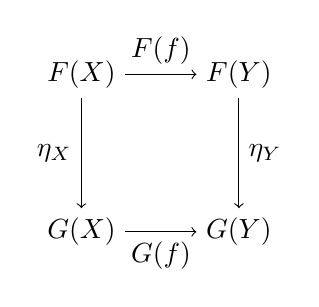
\begin{tikzpicture}
            \node (FX) at (0,0) {\(F(X)\)};
            \node (FY) at (2,0) {\(F(Y)\)};
            \node (GX) at (0,-2) {\(G(X)\)};
            \node (GY) at (2,-2) {\(G(Y)\)};
            \draw[->] (FX) -- node[above] {\(F(f)\)} (FY);
            \draw[->] (FX) -- node[left] {\(\eta_X\)} (GX);
            \draw[->] (FY) -- node[right] {\(\eta_Y\)} (GY);
            \draw[->] (GX) -- node[below] {\(G(f)\)} (GY);
        \end{tikzpicture}
    \end{center}

    记作 \(\eta : F \to G\), 可以画作图表:

    \begin{center}
        \begin{tikzpicture}
            \node (C) at (-2,0) {\(\mathcal{C}\)};
            \node (D) at (2,0) {\(\mathcal{D}\)};
            \draw[->] (C) to[bend left=60] node[above] (F) {\(F\)} (D);
            \draw[->] (C) to[bend right=60] node[below] (G) {\(G\)} (D);
            \draw[double,-{Implies},double distance = 0.15em] ($(F.south) + (0,- 0.1)$) to node[right] {\(\eta\)} ($(G.north) + (0,0.1)$);
        \end{tikzpicture}
    \end{center}
\end{definition}

\begin{definition}[纵合成]
    给出 \(\eta : F \to G\), \(\theta : G \to H\), 定义纵合成 \(\theta \circ \eta : F \to H\) 为 \({(\theta \circ \eta)}_X := \theta_X \circ \eta_X\), 解作图表:
    
    \[
        \begin{tikzpicture}
            \node (C) at (-2,0) {\(\mathcal{C}\)};
            \node (D) at (2,0) {\(\mathcal{D}\)};
            \draw[->] (C) to[bend left=40] node[above] (F) {\(F\)} (D);
            \draw[->] (C) to node[above] (G) {\(G\)} (D);
            \draw[->] (C) to[bend right=40] node[below] (H) {\(H\)} (D);
            \draw[double,-{Implies},double distance = 0.15em] ($(F.south) + (0,- 0.1)$) to node[right] {\(\eta\)} ($(G.north) + (0,0.1)$);
            \draw[double,-{Implies},double distance = 0.15em] ($(G.south) + (0,- 0.1)$) to node[right] {\(\theta\)} ($(H.north) + (0,0.1)$);
        \end{tikzpicture} = \begin{tikzpicture}
            \node (C) at (-2,0) {\(\mathcal{C}\)};
            \node (D) at (2,0) {\(\mathcal{D}\)};
            \draw[->] (C) to[bend left=40] node[above] (F) {\(F\)} (D);
            \draw[->] (C) to[bend right=40] node[below] (H) {\(H\)} (D);
            \draw[double,-{Implies},double distance = 0.15em] ($(F.south) + (0,- 0.1)$) to node[right] {\(\theta \circ \eta\)} ($(H.north) + (0,0.1)$);
        \end{tikzpicture}
    \]

    \begin{proof}
        只需注意到以下交换图表 (两小方块交换故外框交换):

        \begin{center}
            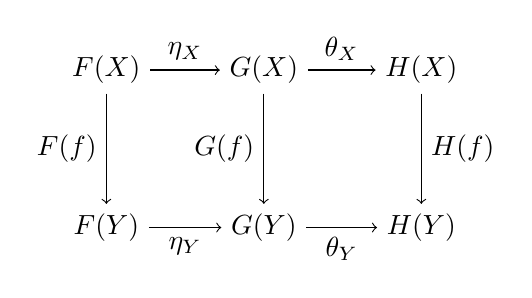
\begin{tikzpicture}
                \node (FX) at (-2,1) {\(F(X)\)};
                \node (FY) at (-2,-1) {\(F(Y)\)};
                \node (GX) at (0,1) {\(G(X)\)};
                \node (GY) at (0,-1) {\(G(Y)\)};
                \node (HX) at (2,1) {\(H(X)\)};
                \node (HY) at (2,-1) {\(H(Y)\)};
                \draw[->] (FX) -- node[left] {\(F(f)\)} (FY);
                \draw[->] (FX) -- node[above] {\(\eta_X\)} (GX);
                \draw[->] (FY) -- node[below] {\(\eta_Y\)} (GY);
                \draw[->] (GX) -- node[left] {\(G(f)\)} (GY);
                \draw[->] (GX) -- node[above] {\(\theta_X\)} (HX);
                \draw[->] (GY) -- node[below] {\(\theta_Y\)} (HY);
                \draw[->] (HX) -- node[right] {\(H(f)\)} (HY);
            \end{tikzpicture}
        \end{center}
    \end{proof}
\end{definition}

\begin{definition}[横合成]
    给出三个范畴 \(\mathcal{C},\mathcal{D},\mathcal{E}\) 以及四个函子 \(F_1,F_2 : \mathcal{C} \to \mathcal{D}\), \(G_1,G_2 : \mathcal{D} \to \mathcal{E}\), 
    给出自然变换 \(\eta : F_1 \to F_2\), \(\theta : G_1 \to G_2\), 定义横合成 \(\theta \ast \eta : G_1 \circ F_1 \to G_2 \circ F_2\) 为 \({(\theta \ast \eta)}_X := \theta_{F_2 (X)} \circ G_1 (\eta_X)\), 解作图表:

    \[
        \begin{tikzpicture}
            \node (C) at (-3,0) {\(\mathcal{C}\)};
            \node (D) at (0,0) {\(\mathcal{D}\)};
            \node (E) at (3,0) {\(\mathcal{E}\)};
            \draw[->] (C) to[bend left=40] node[above] (F1) {\(F_1\)} (D);
            \draw[->] (C) to[bend right=40] node[below] (F2) {\(F_2\)} (D);
            \draw[->] (D) to[bend left=40] node[above] (G1) {\(G_1\)} (E);
            \draw[->] (D) to[bend right=40] node[below] (G2) {\(G_2\)} (E);
            \draw[double,-{Implies},double distance = 0.15em] ($(F1.south) + (0,- 0.1)$) to node[right] {\(\eta\)} ($(F2.north) + (0,0.1)$);
            \draw[double,-{Implies},double distance = 0.15em] ($(G1.south) + (0,- 0.1)$) to node[right] {\(\theta\)} ($(G2.north) + (0,0.1)$);
        \end{tikzpicture} = \begin{tikzpicture}
            \node (C) at (-2,0) {\(\mathcal{C}\)};
            \node (E) at (2,0) {\(\mathcal{E}\)};
            \draw[->] (C) to[bend left=30] node[above] (G1F1) {\(G_1 \circ F_1\)} (E);
            \draw[->] (C) to[bend right=30] node[below] (G2F2) {\(G_2 \circ F_2\)} (E);
            \draw[double,-{Implies},double distance = 0.15em] ($(G1F1.south) + (0,- 0.1)$) to node[right] {\(\theta \ast \eta\)} ($(G2F2.north) + (0,0.1)$);
        \end{tikzpicture}
    \]

    \begin{proof}
        需注意到以下交换图表:

        \begin{center}
            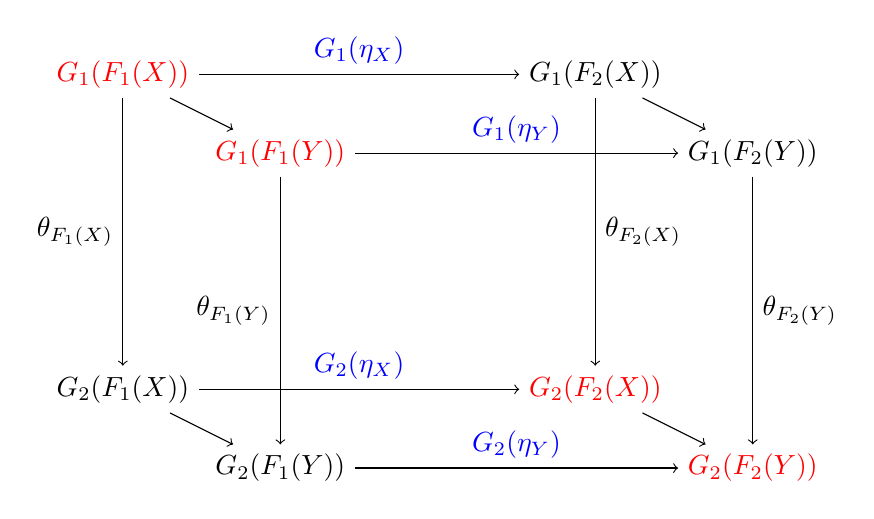
\begin{tikzpicture}
                \node (G1F1X) at (-4,4) {\textcolor{red}{\(G_1 (F_1 (X))\)}};
                \node (G1F1Y) at (-2,3) {\textcolor{red}{\(G_1 (F_1 (Y))\)}};
                \node (G1F2X) at (2,4) {\(G_1 (F_2 (X))\)};
                \node (G1F2Y) at (4,3) {\(G_1 (F_2 (Y))\)};
                \node (G2F1X) at (-4,0) {\(G_2 (F_1 (X))\)};
                \node (G2F1Y) at (-2,-1) {\(G_2 (F_1 (Y))\)};
                \node (G2F2X) at (2,0) {\textcolor{red}{\(G_2 (F_2 (X))\)}};
                \node (G2F2Y) at (4,-1) {\textcolor{red}{\(G_2 (F_2 (Y))\)}};
                \draw[->] (G1F1X) -- (G1F1Y);
                \draw[->] (G1F2X) -- (G1F2Y);
                \draw[->] (G2F1X) -- (G2F1Y);
                \draw[->] (G2F2X) -- (G2F2Y);
                \draw[->] (G1F1X) -- node[above] {\textcolor{blue}{\(G_1 (\eta_X)\)}} (G1F2X);
                \draw[->] (G1F1Y) -- node[above] {\textcolor{blue}{\(G_1 (\eta_Y)\)}} (G1F2Y);
                \draw[->] (G2F1X) -- node[above] {\textcolor{blue}{\(G_2 (\eta_X)\)}} (G2F2X);
                \draw[->] (G2F1Y) -- node[above] {\textcolor{blue}{\(G_2 (\eta_Y)\)}} (G2F2Y);
                \draw[->] (G1F1X) -- node[left] {{\(\theta_{F_1 (X)}\)}} (G2F1X);
                \draw[->] (G1F1Y) -- node[left] {\(\theta_{F_1 (Y)}\)} (G2F1Y);
                \draw[->] (G1F2X) -- node[right] {\(\theta_{F_2 (X)}\)} (G2F2X);
                \draw[->] (G1F2Y) -- node[right] {\(\theta_{F_2 (Y)}\)} (G2F2Y);
            \end{tikzpicture}
        \end{center}

        前后左右四面交换源自 \(\theta\) 为自然变换, 上下两面交换源自 \(\eta\) 为自然变换, 于是\textcolor{red}{红色}标记出的子图亦交换.
    \end{proof}
\end{definition}

特别的, 在标记自然变换时, 我们可以将单独的函子 \(F\) 拉开成为 \(\mathrm{id}_F : F \to F\), 在每个 \(X\) 上为 \(\mathrm{id}_{F(X)}\).

\begin{definition}
    对于范畴 \(\mathcal{C}, \mathcal{D}\), 定义函子范畴 \(\mathbf{Fun} (\mathcal{C},\mathcal{D})\) 如下:

    \begin{enumerate}
        \item 对象是函子 \(\mathcal{C} \to \mathcal{D}\).
        \item 对于函子 \(F,G : \mathcal{C} \to \mathcal{D}\), 定义态射集 \(\mathrm{Hom}_{\mathbf{Fun} (\mathcal{C},\mathcal{D})} (F,G)\) 为所有 \(F \to G\) 的自然变换.
        \item 态射的合成是自然变换的纵合成.
    \end{enumerate}

    \begin{proof}
        只需证明纵合成之结合律, 只需注意到态射结合律:

        \[
            (\theta_X \circ \eta_X) \circ \phi_X = \theta_X \circ (\eta_X \circ \phi_X)
        \]
    \end{proof}
\end{definition}

\begin{lemma}
    函子的纵合成满足结合律.

    \begin{proof}
        给出自然变换 \(\theta, \psi, \phi\) 如下:

        \begin{center}
            \begin{tikzpicture}
                \node (C) at (-3,0) {\(\mathcal{C}\)};
                \node (D) at (-1,0) {\(\mathcal{D}\)};
                \node (E) at (1,0) {\(\mathcal{E}\)};
                \node (F) at (3,0) {\(\mathcal{F}\)};
                \draw[->] (C) to[bend left=40] node[above] (F1) {\(F_1\)} (D);
                \draw[->] (C) to[bend right=40] node[below] (F2) {\(F_2\)} (D);
                \draw[->] (D) to[bend left=40] node[above] (G1) {\(G_1\)} (E);
                \draw[->] (D) to[bend right=40] node[below] (G2) {\(G_2\)} (E);
                \draw[->] (E) to[bend left=40] node[above] (H1) {\(H_1\)} (F);
                \draw[->] (E) to[bend right=40] node[below] (H2) {\(H_2\)} (F);
                \draw[double,-{Implies},double distance = 0.15em] ($(F1.south) + (0,- 0.1)$) to node[right] {\(\eta\)} ($(F2.north) + (0,0.1)$);
                \draw[double,-{Implies},double distance = 0.15em] ($(G1.south) + (0,- 0.1)$) to node[right] {\(\theta\)} ($(G2.north) + (0,0.1)$);
                \draw[double,-{Implies},double distance = 0.15em] ($(H1.south) + (0,- 0.1)$) to node[right] {\(\psi\)} ($(H2.north) + (0,0.1)$);
            \end{tikzpicture}
        \end{center}

        有交换图表 (交换性源自于施 \(\psi\) 自然性于 \(G_2 \eta_X\)):

        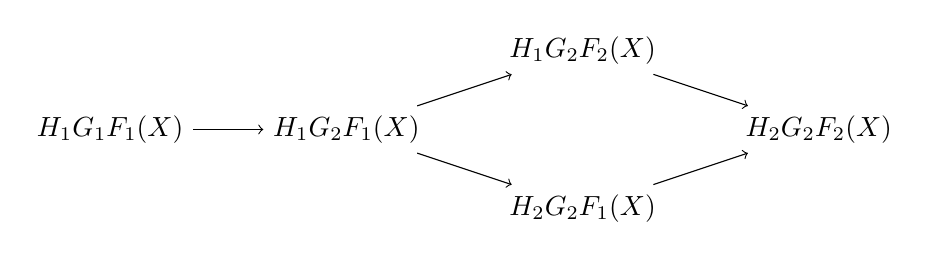
\begin{tikzpicture}
            \node (H1G1F1) at (-4.5,0) {\(H_1 G_1 F_1 (X)\)};
            \node (H1G2F1) at (-1.5,0) {\(H_1 G_2 F_1 (X)\)};
            \node (H1G2F2) at (1.5,1) {\(H_1 G_2 F_2 (X)\)};
            \node (H2G2F2) at (4.5,0) {\(H_2 G_2 F_2 (X)\)};
            \node (H2G2F1) at (1.5,-1) {\(H_2 G_2 F_1 (X)\)};
            \draw[->] (H1G1F1) -- (H1G2F1);
            \draw[->] (H1G2F1) -- (H1G2F2);
            \draw[->] (H1G2F2) -- (H2G2F2);
            \draw[->] (H1G2F1) -- (H2G2F1);
            \draw[->] (H2G2F1) -- (H2G2F2);
        \end{tikzpicture}
    \end{proof}
\end{lemma}

\begin{lemma}
    函子的横纵合成交换, 即亦给出自然变换如下:

    \begin{center}
        \begin{tikzpicture}
            \node (C) at (-3,0) {\(\mathcal{C}\)};
            \node (D) at (0,0) {\(\mathcal{D}\)};
            \node (E) at (3,0) {\(\mathcal{E}\)};
            \draw[->] (C) to[bend left=60] node[above] (F1) {\(F_1\)} (D);
            \draw[->] (C) to node[below] (F2) {\(F_2\)} (D);
            \draw[->] (C) to[bend right=60] node[below] (F3) {\(F_3\)} (D);
            \draw[->] (D) to[bend left=60] node[above] (G1) {\(G_1\)} (E);
            \draw[->] (D) to node[below] (G2) {\(G_2\)} (E);
            \draw[->] (D) to[bend right=60] node[below] (G3) {\(G_3\)} (E);
            \draw[double,-{Implies},double distance = 0.15em] ($(F1.south) + (0,- 0.1)$) to node[right] {\(\eta\)} ($(F2.north) + (0,0.1)$);
            \draw[double,-{Implies},double distance = 0.15em] ($(F2.south)$) to node[right] {\(\eta^\prime\)} ($(F3.north) + (0,0.1)$);
            \draw[double,-{Implies},double distance = 0.15em] ($(G1.south) + (0,- 0.1)$) to node[right] {\(\theta\)} ($(G2.north) + (0,0.1)$);
            \draw[double,-{Implies},double distance = 0.15em] ($(G2.south)$) to node[right] {\(\theta^\prime\)} ($(G3.north) + (0,0.1)$);
        \end{tikzpicture}
    \end{center}

    则有等式 \((\theta^\prime \ast \eta^\prime) \circ (\theta \ast \eta) = (\theta^\prime \circ \theta) \ast (\eta^\prime \circ \eta)\).

    \begin{proof}
        只需注意到以下交换图表:

        \begin{center}
            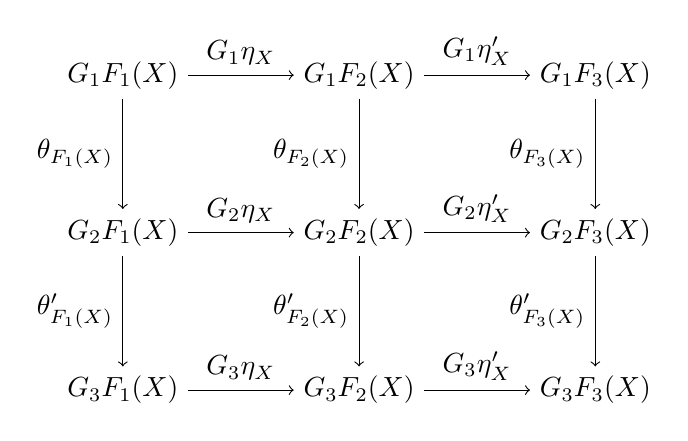
\begin{tikzpicture}
                \node (G1F1X) at (-3,2) {\(G_1 F_1 (X)\)};
                \node (G1F2X) at (0,2) {\(G_1 F_2 (X)\)};
                \node (G1F3X) at (3,2) {\(G_1 F_3 (X)\)};
                \node (G2F1X) at (-3,0) {\(G_2 F_1 (X)\)};
                \node (G2F2X) at (0,0) {\(G_2 F_2 (X)\)};
                \node (G2F3X) at (3,0) {\(G_2 F_3 (X)\)};
                \node (G3F1X) at (-3,-2) {\(G_3 F_1 (X)\)};
                \node (G3F2X) at (0,-2) {\(G_3 F_2 (X)\)};
                \node (G3F3X) at (3,-2) {\(G_3 F_3 (X)\)};
                \draw[->] (G1F1X) to node[above] {\(G_1 \eta_X\)} (G1F2X);
                \draw[->] (G1F2X) to node[above] {\(G_1 \eta^\prime_X\)} (G1F3X);
                \draw[->] (G2F1X) to node[above] {\(G_2 \eta_X\)} (G2F2X);
                \draw[->] (G2F2X) to node[above] {\(G_2 \eta^\prime_X\)} (G2F3X);
                \draw[->] (G3F1X) to node[above] {\(G_3 \eta_X\)} (G3F2X);
                \draw[->] (G3F2X) to node[above] {\(G_3 \eta^\prime_X\)} (G3F3X);
                \draw[->] (G1F1X) to node[left] {\(\theta_{F_1 (X)}\)} (G2F1X);
                \draw[->] (G1F2X) to node[left] {\(\theta_{F_2 (X)}\)} (G2F2X);
                \draw[->] (G1F3X) to node[left] {\(\theta_{F_3 (X)}\)} (G2F3X);
                \draw[->] (G2F1X) to node[left] {\(\theta^\prime_{F_1 (X)}\)} (G3F1X);
                \draw[->] (G2F2X) to node[left] {\(\theta^\prime_{F_2 (X)}\)} (G3F2X);
                \draw[->] (G2F3X) to node[left] {\(\theta^\prime_{F_3 (X)}\)} (G3F3X);
            \end{tikzpicture}
        \end{center}

        每个小正方形交换源于 \(\theta, \theta^\prime\) 为自然变换, 故外框交换.
    \end{proof}
\end{lemma}

\begin{lemma}
    \label {lemma:natural transformation is isomorphism iff each component is isomorphism}
    自然变换 \(\eta : F \to G\) 是同构当且仅当对于任意 \(X \in \mathcal{C}\), \(\eta_X\) 是同构,
    其逆为 \(\eta^{-1} : G \to F\), \(\eta^{-1}_X := {\eta_X}^{-1}\).

    \begin{proof}
        给出其逆业已给出每个 \(\eta_X\) 之逆, 而 \(\eta^{-1}\) 是自然性对应了
        \(\eta\) 自然性的交换图表, 换言之, 以下图表每一小块交换故外框交换.

        \begin{center}
            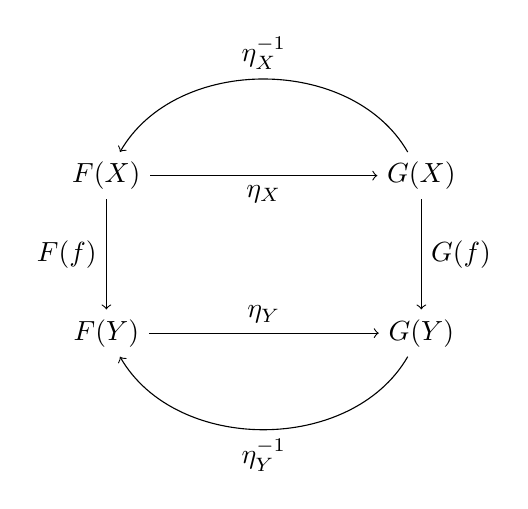
\begin{tikzpicture}
                \node (FX) at (-2,1) {\(F(X)\)};
                \node (FY) at (-2,-1) {\(F(Y)\)};
                \node (GX) at (2,1) {\(G(X)\)};
                \node (GY) at (2,-1) {\(G(Y)\)};
                \draw[->] (FX) to node[left] {\(F(f)\)} (FY);
                \draw[->] (FX) to node[below] {\(\eta_X\)} (GX);
                \draw[->] (FY) to node[above] {\(\eta_Y\)} (GY);
                \draw[->] (GX) to node[right] {\(G(f)\)} (GY);
                \draw[->] (GX) to [bend right=60] node[above] {\(\eta^{-1}_X\)} (FX);
                \draw[->] (GY) to [bend left=60] node[below] {\(\eta^{-1}_Y\)} (FY);
            \end{tikzpicture}
        \end{center}
    \end{proof}
\end{lemma}

\begin{definition}[范畴等价]
    若存在函子 \(F : \mathcal{C} \to \mathcal{D}\), \(G : \mathcal{D} \to \mathcal{C}\) 使得 \(G \circ F \cong \mathrm{id}_{\mathcal{C}}\), \(F \circ G \cong \mathrm{id}_{\mathcal{D}}\), 则称 \(\mathcal{C}\) 与 \(\mathcal{D}\) 等价.

    假定上述定义中 \(\cong\) 为 \(=\), 则称 \(\mathcal{C}\) 与 \(\mathcal{D}\) 同构.
\end{definition}

\begin{definition}[子范畴]
    给定范畴 \(\mathcal{C}^\prime, \mathcal{C}\), 若 \(\mathrm{Ob} (\mathcal{C}^\prime) \subseteq \mathrm{Ob} (\mathcal{C})\), 
    \(\mathrm{Hom}_{\mathcal{C}^\prime} (X,Y) \subseteq \mathrm{Hom}_{\mathcal{C}} (X,Y)\), 且保持复合运算,
    则称 \(\mathcal{C}^\prime\) 是 \(\mathcal{C}\) 的子范畴 (subcategory), 子范畴对应一个自然的嵌入 \(\iota : \mathcal{C}^\prime \to \mathcal{C}\),
    总是忠实, 子范畴亦有全和本质满的性质.
\end{definition}

\begin{definition}[骨架]
    如果范畴 \(\mathcal{C}^\prime\) 是 \(\mathcal{C}\) 的全子范畴, 且对于任意 \(X \in \mathrm{Ob} (\mathcal{C})\),
    都存在唯一 \(X^\prime \in \mathrm{Ob} (\mathcal{C}^\prime)\) 使得 \(X \cong X^\prime\), 则称 \(\mathcal{C}^\prime\) 是 \(\mathcal{C}\) 的骨架 (skeleton).

    自身是骨架的范畴称为骨架范畴 (skeletal category).
\end{definition}

\begin{definition}[小范畴]
    为了避免一些集合论的困难, 我们定义小范畴 (small category) 为态射类是集合的范畴.

    给出一个 Grothendieck 宇宙 \(\mathcal{U}\), 定义 \(\mathcal{U}\)-小范畴为对象类是 \(\mathcal{U}\) 中的集合的范畴.
\end{definition}

\begin{lemma}
    任何小范畴 \(\mathcal{C}\) 有骨架, 且骨架范畴与 \(\mathcal{C}\) 等价.

    \begin{proof}
        注意到 \(\cong\) 显见的是 \(\mathrm{Ob} (\mathcal{C})\) 上的等价关系, 在每个等价类
        上使用 \ref{axiom:NBG Axiom of Choice} 选取代表元 \(X^\prime\), 与等价类中任意一 \(X\) 与 \(X^\prime\) 间同构 \(f_X : X \to X^\prime\),
        选取子范畴 \(\mathcal{C}^\prime\) 如下:

        \begin{enumerate}
            \item 对象集为全体代表元 \(X^\prime\).
            \item 对于任意 \(X^\prime,Y^\prime \in \mathrm{Ob} (\mathcal{C}^\prime)\), \(\mathrm{Hom}_{\mathcal{C}^\prime} (X^\prime,Y^\prime) = \mathrm{Hom}_{\mathcal{C}} (X^\prime,Y^\prime) \).
        \end{enumerate}

        定义 \(\iota^{-1}\) 映 \(X\) 为其代表元 \(X^\prime\), 映 \(f \in \mathrm{Hom}_{\mathcal{C}} (X,Y)\) 为 
        \(f_Y \circ f \circ {f_X}^{-1}\).

        \(\iota^{-1}\) 函子性, \(\iota \circ \iota^{-1} = \mathrm{id}_{\mathcal{C}}\) 是显然的, 而构造 \(\iota^{-1} \circ \iota \cong \mathrm{id}_{\mathcal{C}^\prime}\) 的自然变换为 \(f\) 即可.
    \end{proof}
\end{lemma}

\begin{lemma}
    范畴等价具有传递性.

    \begin{proof}
        给出范畴 \(\mathcal{C},\mathcal{D},\mathcal{E}\), 函子 \(F : \mathcal{C} \to \mathcal{D}\), \(G : \mathcal{D} \to \mathcal{E}\), 
        以及其逆, 给出可逆的自然变换 \(\eta : F \circ F^{-1} \to \mathrm{id}_{\mathcal{D}}\), \(\theta : F^{-1} \circ F \to \mathrm{id}_{\mathcal{C}}\),
        \(\eta^\prime : G \circ G^{-1} \to \mathrm{id}_{\mathcal{E}}\), \(\theta^\prime : G^{-1} \circ G \to \mathrm{id}_{\mathcal{D}}\), 构造自然变换
        \(\eta^\prime \circ (\mathrm{id}_G \ast \eta \ast \mathrm{id}_{G^{-1}}) : G \circ F \circ F^{-1} \circ G^{-1} \to \mathrm{id}_{\mathcal{E}}\) 有逆
        \((\mathrm{id}_G \ast \eta^{-1} \ast \mathrm{id}_{G^{-1}}) \circ {\eta^{\prime}}^{-1}\),  \(\theta\) 侧可同理构造.
    \end{proof}
\end{lemma}

\begin{lemma}
    骨架范畴间的全忠实本质满函子都是同构.

    \begin{proof}
        本质满则在对象集上是双射, 全忠实亦给出每个态射集上的双射.
    \end{proof}
\end{lemma}

\begin{lemma}
    小范畴间函子 \(F\) 是等价当且仅当 \(F\) 全忠实本质满.

    \begin{proof}
        易得骨架范畴间的同构, 考虑等价的传递性即可.
    \end{proof}
\end{lemma}

\subsection{Hom 函子与泛性质}

\begin{definition}
    对于集合 \(I\) 与小范畴 \({(\mathcal{C}_i)}_{i \in I}\), 定义积范畴 \(\prod_{i \in I} \mathcal{C}_i\) 如下:

    \begin{enumerate}
        \item 对象是积 \(\prod_{i \in I} \mathrm{Ob} (\mathcal{C}_i)\) 的元素.
        \item 对于对象 \((X_i)_{i \in I}\), \((Y_i)_{i \in I}\), 定义态射集 \(\mathrm{Hom}_{\prod_{i \in I} \mathcal{C}_i} ((X_i)_{i \in I},(Y_i)_{i \in I})\) 为态射集之积
                \(\prod_{i \in I} \mathrm{Hom}_{\mathcal{C}_i} (X_i,Y_i)\).
        \item 态射的合成是逐点的, 也即 \({(f_i)}_{i \in I} \circ {(g_i)}_{i \in I} = {(f_i \circ g_i)}_{i \in I}\).
    \end{enumerate}

    定义余积范畴 \(\coprod_{i \in I} \mathcal{C}_i\) 如下:

    \begin{enumerate}
        \item 对象是无交并 \(\coprod_{i \in I} \mathrm{Ob} (\mathcal{C}_i)\) 的元素.
        \item 对象 \(X,Y\) 间有态射当且仅当其对应同一个 \(\mathcal{C}_i\), 态射集继承自 \(\mathcal{C}_i\).
    \end{enumerate}

    定义自明的投影函子 \(\mathbf{Pr}_j : \prod_{i \in I} \mathcal{C}_i \to \mathcal{C}_j\) 与包含函子 \(\mathbf{In}_j : \mathcal{C}_j \to \coprod_{i \in I} \mathcal{C}_i\).
\end{definition}

\begin{definition}
    多元函子即为从积范畴出发的函子.
\end{definition}

\begin{definition}[Hom 函子]
    对于任意范畴 \(\mathcal{C}\), 有函子 \(\mathrm{Hom}_{\mathcal{C}} (-,-) : \mathcal{C}^{\mathrm{op}} \times \mathcal{C} \to \mathbf{Set}\), 映 \((X,Y)\) 为态射集 \(\mathrm{Hom}_{\mathcal{C}} (X,Y)\), 
    映 \(\mathcal{C}^{\mathrm{op}} \times \mathcal{C}\) 中态射 \((f,g)\) 为映射 \(\phi \mapsto g \circ \phi \circ f\).

    称 \(\phi\) 对 \(f\) 做拉回 (pullback), 对 \(g\) 做推出 (pushforward).
\end{definition}

\begin{lemma}
    存在自然同构 \({(\mathbf{Fun} (\mathcal{C}_1 ,\mathcal{C}_2))}^\mathrm{op} \cong \mathbf{Fun} ({\mathcal{C}_1}^\mathrm{op}, {\mathcal{C}_2}^\mathrm{op})\).
\end{lemma}

\begin{lemma}
    有恒等式 \(\mathbf{Fun} (\mathrm{Disc} (I), \mathcal{C}) \cong \prod_{i \in I} \mathcal{C}\).
\end{lemma}

\begin{definition}[中心]
    一个范畴的中心定义为 \(\mathrm{Z} (\mathcal{C}) := \mathrm{End} (\mathrm{id}_{\mathcal{C}})\).

    对范畴等价 \(F : \mathcal{C} \to \mathcal{D}\), 诱导出中心的同构 \(\mathrm{Z} (\mathcal{C}) \cong \mathrm{Z} (\mathcal{D})\).
\end{definition}

\begin{definition}
    假设范畴 \(\mathcal{C}\) 中对象 \(X\) 满足任意 \(Y \in \mathrm{Ob} (\mathcal{C})\), \(\mathrm{Hom}_{\mathcal{C}} (X,Y)\) 是单点集, 则称 \(X\) 是始对象 (initial object).
    对称的 \(\mathrm{Hom}_{\mathcal{C}} (Y,X)\) 是单点集的对象称为终对象 (terminal object).既是始对象又是终对象的对象称为零对象 (zero object).
\end{definition}

\begin{example}
    在 \(\mathbf{Set}\) 中, 空集是始对象, 任意单点集是终对象.
\end{example}

\begin{definition}
    始对象间有唯一的同构, 终对象亦然.

    \begin{proof}
        给出始对象 \(X,Y\), 存在唯一的 \(f : X \to Y\), \(g : Y \to X\),
        同样存在唯一的 \(\mathrm{id}_X : X \to X\), \(\mathrm{id}_Y : Y \to Y\), 于是 \(f \circ g = \mathrm{id}_Y\), \(g \circ f = \mathrm{id}_X\).

        终对象只需注意到任意 \(\mathcal{C}\) 的终对象都是 \(\mathcal{C}^{\mathrm{op}}\) 的始对象.
    \end{proof}
\end{definition}

\begin{definition}
    泛性质 (universal property) 是一种在某个范畴下是始对象或终对象的性质, 其有自然的唯一性.
\end{definition}

\begin{definition}[图范畴]
    给出一个图表样式, 定义该图的范畴如下:

    \begin{enumerate}
        \item 对象是所有使得图表交换的一种填涂方式.
        \item 态射是相同位置的对象逐点的态射, 满足生成的柱状图表交换.
    \end{enumerate}
\end{definition}

\begin{example}[态射范畴]
    称下图的图范畴为 \(\mathcal{C}\) 的态射范畴:

    \begin{center}
        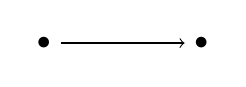
\begin{tikzpicture}
            \node (P1) at (-1,0) {\(\bullet\)};
            \node (P2) at (1,0) {\(\bullet\)};
            \draw[->] (P1) to (P2);
        \end{tikzpicture}
    \end{center}

    即对象是 \(\mathcal{C}\) 中两个对象 \(A,B\) 和一个态射 \(f : A \to B\), 由于确定 \(f\) 亦确定了 \(A,B\),
    也可将对象解作 \(\mathcal{C}\) 中的映射, \(f_1,f_2\) 间的态射是满足以下图表交换的 \((\phi_A, \phi_B)\):

    \begin{center}
        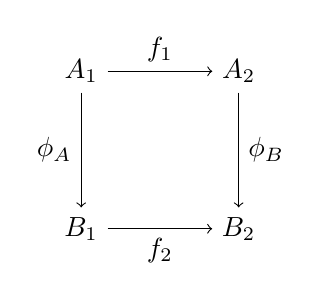
\begin{tikzpicture}
            \node (A1) at (-1,1) {\(A_1\)};
            \node (A2) at (1,1) {\(A_2\)};
            \node (B1) at (-1,-1) {\(B_1\)};
            \node (B2) at (1,-1) {\(B_2\)};
            \draw[->] (A1) to node[above] {\(f_1\)} (A2);
            \draw[->] (B1) to node[below] {\(f_2\)} (B2);
            \draw[->] (A1) to node[left] {\(\phi_A\)} (B1);
            \draw[->] (A2) to node[right] {\(\phi_B\)} (B2);
        \end{tikzpicture}
    \end{center}
\end{example}

\begin{example}[逗号范畴]
    给出函子 \(S : \mathcal{A} \to \mathcal{C}\), \(T : \mathcal{B} \to \mathcal{C}\), 定义逗号范畴 \((S / T)\) 为下图的图范畴:

    \begin{center}
        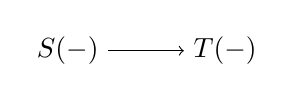
\begin{tikzpicture}
            \node (S) at (-1,0) {\(S (-)\)};
            \node (T) at (1,0) {\(T (-)\)};
            \draw[->] (S) to (T);
        \end{tikzpicture}
    \end{center}

    解作对象是 \(\mathcal{A}\) 中的对象 \(A\), \(\mathcal{B}\) 中的对象 \(B\), 以及 \(\mathcal{C}\) 中的态射 \(f : S(A) \to T(B)\) 组成的 \((A,B,f)\),
    一个 \((A,B,f)\) 到 \((A^\prime,B^\prime,f^\prime)\) 的态射是一对态射 \(g : A \to A^\prime\) 与 \(h : B \to B^\prime\) 使得下图交换:

    \begin{center}
        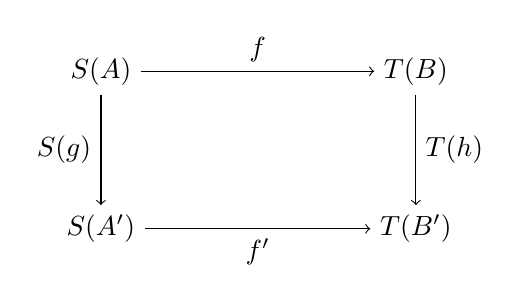
\begin{tikzpicture}
            \node (SA) at (-2,1) {\(S(A)\)};
            \node (TB) at (2,1) {\(T(B)\)};
            \node (SAP) at (-2,-1) {\(S(A^\prime)\)};
            \node (TBP) at (2,-1) {\(T(B^\prime)\)};
            \draw[->] (SA) to node[above] {\(f\)} (TB);
            \draw[->] (SAP) to node[below] {\(f^\prime\)} (TBP);
            \draw[->] (SA) to node[left] {\(S(g)\)} (SAP);
            \draw[->] (TB) to node[right] {\(T(h)\)} (TBP);
        \end{tikzpicture}
    \end{center}
\end{example}

\begin{definition}[子对象, 商对象]
    对 \(X \in \mathrm{Ob} (\mathcal{C})\), 定义 \(X\) 的子对象为单态射 \(i : Y \to X\),
    定义商对象为满态射 \(p : X \to Z\), 在子对象和商对象上定义序:

    定义子对象与商对象的范畴:

    \begin{enumerate}
        \item 对象是 \(X\) 的子对象.
        \item \(i_1 : Y_1 \to X\) 与 \(i_2 : Y_2 \to X\) 的态射是 \(f : Y_1 \to Y_2\) 使得 \(i_1 = i_2 \circ f\).
    \end{enumerate}

    \begin{enumerate}
        \item 对象是 \(X\) 的商对象.
        \item \(p_1 : X \to Z_1\) 与 \(p_2 : X \to Z_2\) 的态射是 \(f : Z_1 \to Z_2\) 使得 \(p_1 = f \circ p_2\).
    \end{enumerate}

    定义子对象与商对象的偏序: \(i_1 \le i_2\) 当且仅当有子对象范畴中的态射 \(f : Y_1 \to Y_2\),
    \(p_1 \le p_2\) 当且仅当有商对象范畴中的态射 \(f : Z_1 \to Z_2\).
\end{definition}

\begin{lemma}
    如果子对象 \(i_1 \le i_2\) 且 \(i_2 \le i_1\), 则子对象 \(i_1\) 与 \(i_2\) 同构, 商对象亦然.

    \begin{proof}
        注意到两个子对象间存在态射则唯一, 于是两个方向均合成为恒等态射.

        商对象无非是 \(\mathcal{C}^{\mathrm{op}}\) 中的子对象.
    \end{proof}
\end{lemma}

\subsection{米田引理}

\begin{definition}[预层]
    给出小范畴 \(\mathcal{C}\), 定义范畴 \(\mathcal{C}^{\vee} : \mathbf{Fun} (\mathcal{C}^{\mathrm{op}}, \mathbf{Set}^{\mathrm{op}})\) 与
    \(\mathcal{C}^{\wedge} : \mathbf{Fun} (\mathcal{C}^{\mathrm{op}}, \mathbf{Set})\), 称 \(\mathcal{C}^{\wedge}\) 为预层 (presheaf) 范畴.
\end{definition}

\begin{definition}
    我们可以自然的将 \(\mathcal{C}\) 嵌入 \(\mathcal{C}^{\wedge}\) 如下:
    \[
        h_{\mathcal{C}} : S \mapsto \mathrm{Hom}_{\mathcal{C}} (-,S)
    \]
    定义自然的求值函子 \(\mathrm{ev}^{\wedge} : \mathcal{C}^{\mathrm{op}} \times \mathcal{C}^{\wedge} \to \mathbf{Set}\) 如下:
    \[
        \mathrm{ev}^{\wedge} (X,S) := S(X)
    \]
    对偶的, 定义 \(k_\mathcal{C} : \mathcal{C} \to \mathcal{C}^{\vee}, \mathrm{ev}^{\vee} : {(\mathcal{C}^{\vee})}^{\mathrm{op}} \times \mathcal{C} \to \mathbf{Set}\) 如下:
    \[
        k_\mathcal{C} (S) := \mathrm{Hom}_{\mathcal{C}} (S,-), \mathrm{ev}^{\vee} (S,X) := S(X)
    \]
\end{definition}

下述引理称米田引理 (Yoneda lemma), 是范畴论中非常重要的引理.

\begin{lemma}[Yoneda]
    \setlabel {米田引理}
    \label {lemma:Yoneda lemma}
    对于任意 \(\mathcal{C}\) 上的预层 \(A \in \mathrm{Ob} (\mathcal{C}^{\wedge})\), 与对象 \(S \in \mathcal{C}\), 
    存在 \(\mathrm{Hom}_{\mathcal{C}^{\wedge}} (h_{\mathcal{C}} (S), A) \cong A(S)\) 的自然双射:
    \[
        (\phi : h_{\mathcal{C}} (S) \to A) \mapsto \phi_S (\mathrm{id}_S)
    \]
    此双射给出 \(\mathrm{Hom}_{\mathcal{C}^{\wedge}} (h_{\mathcal{C}} (-), -)\) 与 \(\mathrm{ev}^{\wedge}\) 的同构.

    \begin{proof}
        证明的技巧在于向层的嵌入将映射转为拉回和推出, 所以对于所有 \(a \in A(S)\), 可以限制出 \(\phi_a : h_{\mathcal{C}} (S) \to A\) 为 \(f \in \mathrm{Hom}_{\mathcal{C}} (X,S)\) 有:
        \[
            \phi_a (f) = \phi_a (\mathrm{id}_S \circ f) = \phi_a (((h_{\mathcal{C}} (S)) (f)) (\mathrm{id}_S)) = A(f) \phi_a (\mathrm{id}_S) = A(f) (a)
        \]
        \begin{center}
            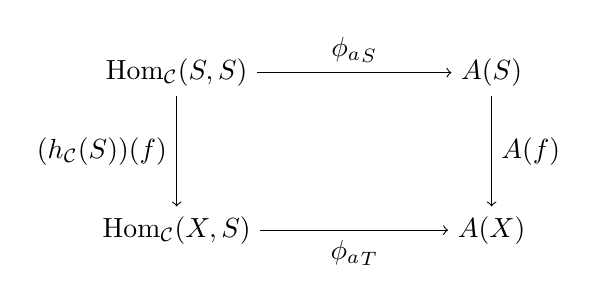
\begin{tikzpicture}
                \node (HSS) at (-2,1) {\(\mathrm{Hom}_{\mathcal{C}} (S,S)\)};
                \node (HXS) at (-2,-1) {\(\mathrm{Hom}_{\mathcal{C}} (X,S)\)};
                \node (AS) at (2,1) {\(A(S)\)};
                \node (AX) at (2,-1) {\(A(X)\)};
                \draw[->] (HSS) to node[left] {\((h_{\mathcal{C}} (S)) (f)\)} (HXS);
                \draw[->] (AS) to node[right] {\(A(f)\)} (AX);
                \draw[->] (HSS) to node[above] {\({\phi_a}_S\)} (AS);
                \draw[->] (HXS) to node[below] {\({\phi_a}_T\)} (AX);
            \end{tikzpicture}
        \end{center}

        自然性展开符号即可, 同构基于 \ref{lemma:natural transformation is isomorphism iff each component is isomorphism}.
    \end{proof}
\end{lemma}

\begin{lemma}
    上述 \(h_\mathcal{C}\) 是全忠实函子, 给出了自然的嵌入 \(\mathcal{C} \to \mathcal{C}^{\wedge}\).

    \begin{proof}
        全忠实性考虑取 \(A\) 为 \(h_\mathcal{C}(T)\), \ref{lemma:Yoneda lemma} 即给出 \(\mathrm{Hom}_{\mathcal{C}^{\wedge}} (h_{\mathcal{C}} (S), h_{\mathcal{C}} (T))\), \(\mathrm{Hom}_{\mathcal{C}} (S,T)\)
        间双射.
    \end{proof}
\end{lemma}

\begin{corollary}
    对称的, \(k_\mathcal{C}\) 全忠实, 且有自然的函子同构 \(\mathrm{Hom}_{\mathcal{C}^{\vee}} (k_{\mathcal{C}} (-), -) \to \mathrm{ev}^{\vee}\).

    \begin{proof}
        只需注意到恒等式 \({(\mathcal{C}^{\vee})}^\mathrm{op} = {(\mathcal{C}^{\mathrm{op}})}^{\wedge}\).
    \end{proof}
\end{corollary}

\begin{definition}[可表]
    称预层 \(A\) 可表 (representable) 当且仅当存在对象 \(S \in \mathcal{C}\) 并给出 \(A \cong h_{\mathcal{C}} (S)\) 的同构 \(\phi : h_{\mathcal{C}} (S) \to A\),
    并称 \((S,\phi)\) 是 \(A\) 的代表元, 对 \(B \in \mathbf{Fun} (\mathcal{C},\mathbf{Set})\) 亦然.
\end{definition}

\begin{lemma}
    代表元若存在则在同构意义下唯一.

    \begin{proof}
        利用米田嵌入的全忠实性.
    \end{proof}
\end{lemma}

\subsection{伴随对}

\begin{definition}[伴随]
    给出函子 \(F : \mathcal{C} \to \mathcal{D}\), \(G : \mathcal{D} \to \mathcal{C}\), 
    与自然变换 \(\eta : \mathrm{id}_{\mathcal{C}} \to G \circ F\), \(\varepsilon : F \circ G \to \mathrm{id}_{\mathcal{D}}\),
    使得以下两图表合成为恒等自然变换:

    \begin{center}
        \begin{tikzpicture}
            \node (C1) at (-0.5,0.5) {\(\mathcal{C}\)};
            \node (C2) at (1.5,0.5) {\(\mathcal{C}\)};
            \node (D1) at (-1.5,-0.5) {\(\mathcal{D}\)};
            \node (D2) at (0.5,-0.5) {\(\mathcal{D}\)};
            \draw[->] (C1) to node[above] (idc) {\(\mathrm{id}_{\mathcal{C}}\)} (C2);
            \draw[->] (D1) to node[below] (idd) {\(\mathrm{id}_{\mathcal{D}}\)} (D2);
            \draw[->] (D1) to node[above left] {\(G\)} (C1);
            \draw[->] (D2) to node[below right] {\(G\)} (C2);
            \draw[->] (C1) to node[above right] {\(F\)} (D2);
            \draw[-{Implies},double,double distance = 0.15em] (C1) to node[left] {\(\varepsilon\)} ($(idd.north) + (0,0.1)$);
            \draw[-{Implies},double,double distance = 0.15em] ($(idc.south) + (0,-0.1)$) to node[right] {\(\eta\)} (D2);
        \end{tikzpicture} \begin{tikzpicture}
            \node (C1) at (-1.5,0.5) {\(\mathcal{C}\)};
            \node (C2) at (0.5,0.5) {\(\mathcal{C}\)};
            \node (D1) at (-0.5,-0.5) {\(\mathcal{D}\)};
            \node (D2) at (1.5,-0.5) {\(\mathcal{D}\)};
            \draw[->] (C1) to node[above] (idc) {\(\mathrm{id}_{\mathcal{C}}\)} (C2);
            \draw[->] (D1) to node[below] (idd) {\(\mathrm{id}_{\mathcal{D}}\)} (D2);
            \draw[->] (C1) to node[below left] {\(F\)} (D1);
            \draw[->] (C2) to node[above right] {\(F\)} (D2);
            \draw[->] (D1) to node[below right] {\(G\)} (C2);
            \draw[-{Implies},double,double distance = 0.15em] (C2) to node[right] {\(\varepsilon\)} ($(idd.north) + (0,0.1)$);
            \draw[-{Implies},double,double distance = 0.15em] ($(idc.south) + (0,-0.1)$) to node[left] {\(\eta\)} (D1);
        \end{tikzpicture}
    \end{center}

    写成合成为:

    \[
        (\mathrm{id}_{G} \ast \varepsilon) \circ (\eta \ast \mathrm{id}_{G}) = \mathrm{id}_{G}, (\varepsilon \ast \mathrm{id}_{F}) \circ (\mathrm{id}_{F} \ast \eta) = \mathrm{id}_{F}
    \]

    称 \(F\) 为 \(G\) 的左伴随 (left adjoint), \(G\) 为 \(F\) 的右伴随 (right adjoint), 记为 \(F \dashv G\).
\end{definition}

\begin{lemma}
    \(F\) 是 \(G\) 左伴随当且仅当有 \(\mathcal{C}^{\mathrm{op}} \times \mathcal{D} \to \mathbf{Set}\) 中函子
    \(\mathrm{Hom}_{\mathcal{D}} (F (-), -)\) 与 \(\mathrm{Hom}_{\mathcal{C}} (-, G (-))\) 同构.

    \begin{proof}
        我们的任务是找到这样一个一一对应, 这里的技术在于把映射变成拉回推出.

        假定我们给出伴随函子 \(F,G\) 和 \(f \in \mathrm{Hom}_{\mathcal{D}} (F (X), Y)\), 构造
        \(\varphi(f) : X \to G (Y)\) 为 \(G (f) \circ \eta_X\); 对 \(g \in \mathrm{Hom}_{\mathcal{C}} (X, G(Y))\) 构造
        \(\varphi^{-1} (g) : F(X) \to Y\) 为 \(\varepsilon_Y \circ F (g)\).

        而 \(\varphi^{-1} \varphi (f) = \varepsilon_{Y} \circ F (G (f) \circ \eta_X) = (\varepsilon_Y \circ FG f) \circ \eta_X = f \circ \varepsilon_{F(X)} \circ F (\eta_X) = f\),
        \(\varphi \varphi^{-1} (g) = G(\varepsilon_Y \circ F(g)) \circ \eta_X = G (\varepsilon_Y) \circ (GF (g) \circ \eta_{X}) = G (\varepsilon_Y) \circ \eta_{G(Y)} \circ g = g\).

        接下来验证 \(\varphi\) 自然性, \(\varphi(a \circ f \circ F(b)) = G(a) \circ G(f) \circ GF (b) \circ \eta_{X^\prime} = G(a) \circ G(f) \circ \eta_X \circ b\),
        \(\varphi^{-1} (G(a) \circ g \circ b) = \varepsilon_{Y^\prime} \circ FG(a) \circ F(g) \circ F(b) = a \circ \varepsilon_Y \circ F(g) \circ F(b)\).

        反之, 给出 \(\varphi\) 与 \(\varphi^{-1}\), 定义 \(\eta_X := \varphi (\mathrm{id}_{F(X)})\), \(\varepsilon_Y := \varphi^{-1} (\mathrm{id}_{G(Y)})\),
        自然性继承自 \(\varphi\) 与 \(\varphi^{-1}\) 的自然性.

        需验证上述自然变换合成等式 \(G \varepsilon_Y \circ \eta_{G(Y)} = \varphi \varphi^{-1} (\mathrm{id}_{G(Y)} \circ \mathrm{id}_{FGY}) = \mathrm{id}_{G(Y)}\),
        \(\varepsilon_{F(X)} \circ F \eta_X = \varphi^{-1} \varphi (\mathrm{id}_{F(X)} \circ \mathrm{id}_{F \eta_X}) = \mathrm{id}_{F(X)}\).
    \end{proof}
\end{lemma}

上述引理给出了伴随对在 \(\mathrm{Hom}\) 集上的体现, 于是我们可以考虑伴随与可表的关系.

\begin{lemma}
    函子 \(F : \mathcal{C} \to \mathcal{D}\) 有右伴随当且仅当 \(\mathrm{Hom}_{\mathcal{D}} (F (-), Y)\) 对每个 \(Y\) 皆可表.

    \begin{proof}
        我们利用可表函子显式的逐点表示出 \(G\).

        对任意 \(Y\), 假定上述函子被 \((S_Y, \phi_Y)\) 表, 则构造出函子 \(G\) 使得 \(G(Y) = S_Y\),
        对于映射 \(f : Y \to Y^\prime\), 令 \(G(f) : S_Y \to S_{Y^\prime}\) 为与 \({\phi_{Y^\prime}}^{-1} \circ h_{\mathcal{C}} (f) \circ \phi_Y \in \mathrm{Mor} (\mathcal{C}^{\wedge})\)
        对应的唯一映射, 则函子性自然归结于 \(h_\mathcal{C}\) 的函子性.

        注意到 \({(\phi_Y)}_X\) 自然给出了 \(\mathrm{Hom}_{\mathcal{D}} (F (X), Y) \to \mathrm{Hom}_{\mathcal{C}} (X, G(Y))\),
        而用 \(\phi\) 在 \(X\) 处自然性源于 \(\phi_Y\) 的自然性, 在 \(Y\) 处自然性源于 \(G(f)\) 定义确保了在 \(\mathcal{C}^{\wedge}\) 中的自然性, 亦 \(\mathcal{C}\) 中的自然性.
    \end{proof}
\end{lemma}

\begin{corollary}
    同理, \(G\) 有左伴随当且仅当 \(\mathrm{Hom}_{\mathcal{C}} (X, G (-))\) 对每个 \(X\) 皆可表.
\end{corollary}

\begin{lemma}
    一个函子的左伴随若存在则在同构意义下唯一, 右伴随亦然.

    \begin{proof}
        运用上题的想法, 既已给出了 \(\mathcal{C}^{\wedge}\) 中的同构, 则亦是 \(\mathcal{C}\) 中的同构,
        该同构自然性亦通过 \(\mathcal{C}^{\wedge}\) 中保存.
    \end{proof}
\end{lemma}

\begin{lemma}
    给出范畴 \(\mathcal{C}_1, \mathcal{C}_2, \mathcal{C}_3\), 与函子 \(F : \mathcal{C}_1 \to \mathcal{C}_2\), \(G : \mathcal{C}_2 \to \mathcal{C}_1\),
    \(F^\prime : \mathcal{C}_2 \to \mathcal{C}_3\), \(G^\prime : \mathcal{C}_3 \to \mathcal{C}_2\), 使得 \(F \dashv G\), \(F^\prime \dashv G^\prime\),
    则 \(F^\prime \circ F \dashv G \circ G^\prime\).

    \begin{center}
        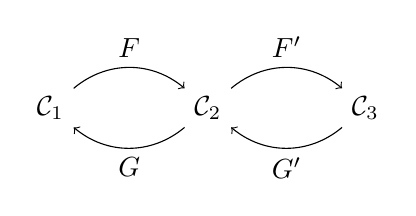
\begin{tikzpicture}
            \node (C1) at (-2,0) {\(\mathcal{C}_1\)};
            \node (C2) at (0,0) {\(\mathcal{C}_2\)};
            \node (C3) at (2,0) {\(\mathcal{C}_3\)};
            \draw[->] (C1) to [bend left = 40] node[above] {\(F\)} (C2);
            \draw[->] (C2) to [bend left = 40] node[above] {\(F^\prime\)} (C3);
            \draw[->] (C2) to [bend left = 40] node[below] {\(G\)} (C1);
            \draw[->] (C3) to [bend left = 40] node[below] {\(G^\prime\)} (C2);
        \end{tikzpicture}
    \end{center}

    \begin{proof}
        给出伴随对应的自然变换 \(\eta, \eta^\prime, \varepsilon, \varepsilon^\prime\),
        定义 \(\xi := (\mathrm{id}_G \ast \eta^\prime \mathrm{id}_{F}) \circ \eta\),
        \(\zeta := \varepsilon^\prime \ast (\varepsilon \ast \mathrm{id}_{G^\prime}) \circ \mathrm{id}_F\),

        \(\xi, \zeta\) 给出 \(F^\prime \circ F \dashv G \circ G^\prime\), 观察以下图表:

        \begin{center}
            \begin{tikzpicture}
                \node (C11) at (-1,1) {\(\mathcal{C}_1\)};
                \node (C12) at (3,1) {\(\mathcal{C}_1\)};
                \node (C21) at (-2,0) {\(\mathcal{C}_2\)};
                \node (C22) at (0,0) {\(\mathcal{C}_2\)};
                \node (C23) at (2,0) {\(\mathcal{C}_2\)};
                \node (C31) at (-3,-1) {\(\mathcal{C}_3\)};
                \node (C32) at (1,-1) {\(\mathcal{C}_3\)};
                \draw[->] (C11) to node[above] (idc1) {\(\mathrm{id}_{\mathcal{C}_1}\)} (C12);
                \draw[->] (C21) to node (idc21) {\(\mathrm{id}_{\mathcal{C}_2}\)} (C22);
                \draw[->] (C22) to node (idc22) {\(\mathrm{id}_{\mathcal{C}_2}\)} (C23);
                \draw[->] (C31) to node[below] (idc3) {\(\mathrm{id}_{\mathcal{C}_3}\)} (C32);
                \draw[->] (C31) to node[above left] {\(G^\prime\)} (C21);
                \draw[->] (C21) to node[above left] {\(G\)} (C11);
                \draw[->] (C11) to node[above right] {\(F\)} (C22);
                \draw[->] (C22) to node[below left] {\(F^\prime\)} (C32);
                \draw[->] (C32) to node[below right] {\(G^\prime\)} (C23);
                \draw[->] (C23) to node[below right] {\(G\)} (C12);
                \draw[-{Implies},double,double distance = 0.15em] (C11) to node[left] {\(\eta\)} (idc21);
                \draw[-{Implies},double,double distance = 0.15em] (idc21) to node[right] {\(\eta^\prime\)} ($(idc3.north) + (0,0.1)$);
                \draw[-{Implies},double,double distance = 0.15em] (idc22) to node[left] {\(\varepsilon^\prime\)} (C32);
                \draw[-{Implies},double,double distance = 0.15em] ($(idc1.south) + (0,-0.1)$) to node[right] {\(\varepsilon\)} (idc22);
            \end{tikzpicture}
        \end{center}

        此图表合成 \(\mathrm{id}_{G \circ G^\prime}\) 只需注意到上下两个平行四边形均合成单位自然变换, 而左右两个大三角形分别代表 \(\xi, \zeta\),
        另一个图表同理合成 \(\mathrm{id}_{F^\prime \circ F}\).
    \end{proof}
\end{lemma}

\begin{definition}
    我们定义 \(2\) - 范畴为满足如下条件的范畴:

    \begin{enumerate}
        \item 一个范畴 \(\mathcal{C}\).
        \item 任取 \(X,Y \in \mathrm{Ob} (\mathcal{C})\), 有范畴 \(\mathcal{D}\) 使得 \(\mathrm{Mor} (\mathcal{D}) = \mathrm{Hom}_\mathcal{C} (X,Y)\).
        \item 有横合成, 给出 \(f, f^\prime \in \mathrm{Hom}_\mathcal{C} (X,Y)\), \(g, g^\prime \in \mathrm{Hom}_\mathcal{C} (Y,Z)\), 与
                \(2\) - 态射 \(\phi : f \to f^\prime\), \(\psi : g \to g^\prime\), 存在态射 \(\phi \ast \psi : g \circ f \to g^\prime \circ f^\prime\).
        \item 横合成结合, 且与纵合成交换.
        \item 两个单位横合成仍是单位.
    \end{enumerate}
\end{definition}

记原范畴的元素为 \(\mathrm{Mor}_0\), 原范畴的态射为 \(\mathrm{Mor}_1\), 称 \(1\) - 态射, \(2\) - 态射记为 \(\mathrm{Mor}_2\).

\begin{example}
    \(\mathbf{Cat}\) 是 \(2\) - 范畴, 对象是全体范畴, 态射是范畴间的函子, \(2\) - 态射是自然变换.
\end{example}

我们可以绘制 \(2\) - 范畴对应的图表, 用 \(\Rightarrow\) 表示 \(2\) - 态射, 依旧用 \(\mathrm{Hom}\) 表示两点间态射对应的范畴.

\begin{definition}[Kan 延拓]
    在 \(2\) - 范畴 \(\Theta\) 中给出对象 \(\mathcal{C},\mathcal{D},\mathcal{E} \in \mathrm{Mor}_0 (\Theta)\),
    给出 \(1\) - 态射 \(F : \mathcal{C} \to \mathcal{E}, K : \mathcal{C} \to \mathcal{D}\).

    定义左 Kan 延拓 \(\mathrm{Lan}_K F : \mathcal{D} \to \mathcal{E}\) 与其对应的 \(2\) - 态射 \(\eta : F \to \mathrm{Lan}_K F \circ K\),
    满足任给 \(G : \mathcal{D} \to \mathcal{E}\) 与 \(2\) - 态射 \(\phi : F \to G \circ K\), 存在唯一的 \(2\) - 态射 \(\phi^\prime : \mathrm{Lan}_K F \to G\), 满足以下等式:

    \[
        \begin{tikzpicture}
            \node (C) at (-2,2) {\(\mathcal{C}\)};
            \node (D) at (0,0) {\(\mathcal{D}\)};
            \node (E) at (2,2) {\(\mathcal{E}\)};
            \draw[->] (C) to node[above] (F) {\(F\)} (E);
            \draw[->] (C) to node[below left] {\(K\)} (D);
            \draw[->] (D) to [bend right = 60] node[below right] (G) {\(G\)} (E);
            \draw[->] (D) to node (Lan) {\(\mathrm{Lan}_K F\)} (E);
            \draw[-{Implies},double,double distance = 0.15em] ($(F.south) + (0 , - 0.1)$) to node[left] {\(\eta\)} (D);
            \draw[-{Implies},double,double distance = 0.15em] (Lan) to node[below left] {\(\phi^\prime\)} (G);
        \end{tikzpicture} = \begin{tikzpicture}
            \node (C) at (-2,2) {\(\mathcal{C}\)};
            \node (D) at (0,0) {\(\mathcal{D}\)};
            \node (E) at (2,2) {\(\mathcal{E}\)};
            \draw[->] (C) to node[above] (F) {\(F\)} (E);
            \draw[->] (C) to node[below left] {\(K\)} (D);
            \draw[->] (D) to node[below right] (G) {\(G\)} (E);
            \draw[-{Implies},double,double distance = 0.15em] ($(F.south) + (0 , - 0.1)$) to node[left] {\(\phi\)} (D);
        \end{tikzpicture}
    \]

    对偶的, 定义右 Kan 延拓 \(\mathrm{Ran}_K F : \mathcal{D} \to \mathcal{E}\) 与其对应的 \(2\) - 态射 \(\varepsilon : \mathrm{Ran}_K F \circ K \to F\),
    满足任给 \(G : \mathcal{D} \to \mathcal{E}\) 与 \(2\) - 态射 \(\phi : G \circ K \to F\), 存在唯一的 \(2\) - 态射 \(\phi^\prime : G \to \mathrm{Ran}_K F\), 满足以下等式:

    \[
        \begin{tikzpicture}
            \node (C) at (-2,2) {\(\mathcal{C}\)};
            \node (D) at (0,0) {\(\mathcal{D}\)};
            \node (E) at (2,2) {\(\mathcal{E}\)};
            \draw[->] (C) to node[above] (F) {\(F\)} (E);
            \draw[->] (C) to node[below left] {\(K\)} (D);
            \draw[->] (D) to [bend right = 60] node[below right] (G) {\(G\)} (E);
            \draw[->] (D) to node (Ran) {\(\mathrm{Ran}_K F\)} (E);
            \draw[-{Implies},double,double distance = 0.15em] (D) to node[above left] {\(\varepsilon\)} ($(F.south) + (0 , - 0.1)$);
            \draw[-{Implies},double,double distance = 0.15em] (G) to node[below left] {\(\phi^\prime\)} (Ran);
        \end{tikzpicture} = \begin{tikzpicture}
            \node (C) at (-2,2) {\(\mathcal{C}\)};
            \node (D) at (0,0) {\(\mathcal{D}\)};
            \node (E) at (2,2) {\(\mathcal{E}\)};
            \draw[->] (C) to node[above] (F) {\(F\)} (E);
            \draw[->] (C) to node[below left] {\(K\)} (D);
            \draw[->] (D) to node[below right] (G) {\(G\)} (E);
            \draw[-{Implies},double,double distance = 0.15em] (D) to node[above left] {\(\phi\)} ($(F.south) + (0 , - 0.1)$);
        \end{tikzpicture}
    \]
\end{definition}

\begin{lemma}
    Kan 延拓存在则在同构意义下唯一.

    \begin{proof}
        利用泛性质唯一性.
    \end{proof}
\end{lemma}

\begin{lemma}
    如若所有 \(F : \mathcal{C} \to \mathcal{E}\) 的右 Kan 延拓存在, 则 \(\mathrm{Ran}_K\) 给出
    从 \(\mathrm{Hom} (\mathcal{C}, \mathcal{E})\) 到 \(\mathrm{Hom} (\mathcal{D}, \mathcal{E})\) 的函子.

    \begin{proof}
        需给出 \(\mathrm{Ran}_K\) 对态射的作用, 给出 \(F \to G\) 的态射 \(\phi : F \to G\), 定义 \(\mathrm{Ran}_K \phi\) 为使得以下等式成立的唯一态射:

        \[
            \begin{tikzpicture}
                \node (C) at (-2,2) {\(\mathcal{C}\)};
                \node (D) at (0,0) {\(\mathcal{D}\)};
                \node (E) at (2,2) {\(\mathcal{E}\)};
                \draw[->] (C) to node[above] (F) {\(F\)} (E);
                \draw[->] (C) to [bend left = 60] node[above] (G) {\(G\)} (E);
                \draw[->] (C) to node[below left] {\(K\)} (D);
                \draw[->] (D) to node (Ran) {\(\mathrm{Ran}_K F\)} (E);
                \draw[-{Implies},double,double distance = 0.15em] (D) to node[left] {\(\varepsilon\)} ($(F.south) + (0 , - 0.1)$);
                \draw[-{Implies},double,double distance = 0.15em] (F) to node[left] {\(\phi\)} ($(G.south) + (0 , - 0.1)$);
            \end{tikzpicture} = \begin{tikzpicture}
                \node (C) at (-2,2) {\(\mathcal{C}\)};
                \node (D) at (0,0) {\(\mathcal{D}\)};
                \node (E) at (2,2) {\(\mathcal{E}\)};
                \draw[->] (C) to node[above] (G) {\(G\)} (E);
                \draw[->] (C) to node[below left] {\(K\)} (D);
                \draw[->] (D) to [bend left = 40] node (RanG) {\(\mathrm{Ran}_K G\)} (E);
                \draw[->] (D) to [bend right = 60] node (RanF) {\(\mathrm{Ran}_K F\)} (E);
                \draw[-{Implies},double,double distance = 0.15em] (RanF) to node {\(\mathrm{Ran}_K \phi\)} (RanG);
                \draw[-{Implies},double,double distance = 0.15em] (D) to node[above left] {\(\varepsilon\)} ($(G.south) + (0 , - 0.1)$);
            \end{tikzpicture}
        \]

        函子性由唯一性保证.
    \end{proof}
\end{lemma}

\begin{corollary}
    同理, 假定对于所有 \(F : \mathcal{C} \to \mathcal{E}\) 的左 Kan 延拓存在, 则 \(\mathrm{Lan}_K\) 也给出
    从 \(\mathrm{Hom} (\mathcal{C}, \mathcal{E})\) 到 \(\mathrm{Hom} (\mathcal{D}, \mathcal{E})\) 的函子.
\end{corollary}

\begin{lemma}
    有伴随对 \(\mathrm{Lan}_K \dashv (- \circ K) \dashv \mathrm{Ran}_K\), 其中 \((- \circ K)\) 
    定义为将 \(1\) - 态射合成 \(K\), 而将 \(2\) - 态射横合成 \(\mathrm{id}_K\).

    \begin{proof}
        态射集 \(\mathrm{Hom}_{\mathrm{Hom} (\mathcal{D}, \mathcal{E})} (\mathrm{Lan}_K (F),G) \to \mathrm{Hom}_{\mathrm{Hom} (\mathcal{C}, \mathcal{E})} (F,G \circ K)\)
        无非是定义的复写. 在 \(F\) 处自然性是按 \(\mathrm{Lan}_K\) 对态射变换的定义, 在  \(G\) 处的自然性依赖唯一性.
    \end{proof}
\end{lemma}

\begin{lemma}
    在 \(\mathbf{Cat}\) 中考虑, 伴随对 \(F \dashv G\) 给出 Kan 延拓 \(G = \mathrm{Lan}_F (\mathrm{id}_\mathcal{C})\), \(F = \mathrm{Ran}_G (\mathrm{id}_\mathcal{C})\).

    \begin{proof}
        观察下图的合成

        \begin{center}
            \begin{tikzpicture}
                \node (C1) at (-3,1) {\(\mathcal{C}\)};
                \node (C2) at (0,1) {\(\mathcal{C}\)};
                \node (C3) at (3,1) {\(\mathcal{C}\)};
                \node (D1) at (-1.5,-1) {\(\mathcal{D}\)};
                \node (D2) at (1.5,-1) {\(\mathcal{D}\)};
                \draw[->] (C1) to node[above] (idc1) {\(\mathrm{id}_{\mathcal{C}}\)} (C2);
                \draw[->] (C2) to node[above] (idc2) {\(\mathrm{id}_{\mathcal{C}}\)} (C3);
                \draw[->] (D1) to node[below] (idd) {\(\mathrm{id}_{\mathcal{D}}\)} (D2);
                \draw[->] (C1) to node[below left] {\(F\)} (D1);
                \draw[->] (C2) to node[below left] {\(F\)} (D2);
                \draw[->] (D1) to node[below right] {\(G\)} (C2);
                \draw[->] (D2) to node[below right] {\(H\)} (C3);
                \draw[-{Implies},double,double distance = 0.15em] ($(idc1.south) + (0,-0.1)$) to (D1);
                \draw[-{Implies},double,double distance = 0.15em] (C2) to ($(idd.north) + (0,0.1)$);
                \draw[-{Implies},double,double distance = 0.15em] ($(idc2.south) + (0,-0.1)$) to (D2);
            \end{tikzpicture}
        \end{center}

        所需 \(2\) 态射为右侧平行四边形, 另一个方向亦然.
    \end{proof}
\end{lemma}

\subsection{极限}

定义 \(\mathbf{1}\) 为最简单的范畴, 仅有一个对象与一个态射, 记为 \(\bullet\), 任何
范畴都有唯一的函子 \(\mathbf{1} \to \mathcal{C}\).

\begin{definition}[极限]
    在范畴 \(\mathbf{Cat}\) 中考虑.
    
    给出小范畴 \(I\) 与函子 \(F : I \to \mathcal{C}\), \(K : I \to \mathbf{1}\), 
    若 \(\mathrm{Ran}_K F\) 存在, 则称 \(\mathrm{Ran}_K F\) 为 \(F\) 的极限 (limit), 记为 \(\varprojlim F\),
    对称的 \(\mathrm{Lan}_K F\) 称为 \(F\) 的余极限 (colimit), 记为 \(\varinjlim F\), 称 \(I^\mathrm{op}\) 为极限对应的指标, \(I\) 为余极限对应的指标.
\end{definition}

解释一下上述对于极限的定义, 给出一个 \(\mathbf{1}\) 出发的函子, 即选中了 \(\mathcal{C}\) 中的一个对象 (此对象沿用上述符号记作 \(\varprojlim F\) 或 \(\varinjlim F\)),
极限构造中上述 Kan 延拓给出的自然变换标记了从该对象出发的函子到 \(F I\) 中一对象的态射, 满足对于任意 \(f \in \mathrm{Mor}(I)\), 下图交换:

\begin{center}
    \begin{tikzpicture}
        \node (FX) at (-2,2) {\(F X\)};
        \node (FY) at (2,2) {\(F Y\)};
        \node (lim) at (0,0) {\(\varprojlim F\)};
        \draw[->] (FX) to node[above] (Ff) {\(F f\)} (FY);
        \draw[->] (lim) to (FX);
        \draw[->] (lim) to (FY);
    \end{tikzpicture}
\end{center}

Kan 延拓的性质也就被解为, 对于任意给出的 \(L \in \mathcal{C}\), 一族态射 \(\phi_X : L \to F X\), 使得对于任意 \(f \in \mathrm{Mor}(I)\), 下图交换:

\begin{center}
    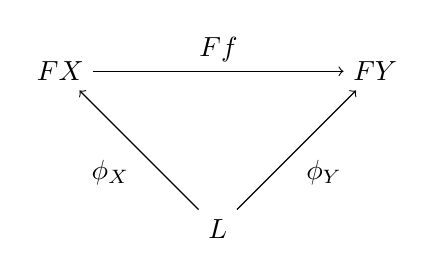
\begin{tikzpicture}
        \node (FX) at (-2,2) {\(F X\)};
        \node (FY) at (2,2) {\(F Y\)};
        \node (L) at (0,0) {\(L\)};
        \draw[->] (FX) to node[above] (Ff) {\(F f\)} (FY);
        \draw[->] (L) to node[below left] (phiX) {\(\phi_X\)} (FX);
        \draw[->] (L) to node[below right] (phiY) {\(\phi_Y\)} (FY);
    \end{tikzpicture}
\end{center}

都有唯一的态射 \(\phi_f : L \to \varprojlim F\), 使得对于任意 \(X \in \mathrm{Ob} (I)\) 下图交换:

\begin{center}
    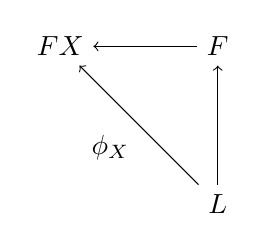
\begin{tikzpicture}
        \node (FX) at (-2,2) {\(F X\)};
        \node (L) at (0,0) {\(L\)};
        \node (lim) at (0,2) {\(\varprojlim F\)};
        \draw[->] (lim) to (FX);
        \draw[->] (L) to node[below left] (phiX) {\(\phi_X\)} (FX);
        \draw[->] (L) to (lim);
    \end{tikzpicture}
\end{center}

余极限将上述所有箭头反向即可得到.

\begin{definition}
    直积 (product) 与余积 (coproduct) 是极限与余极限的特例, 分别对应于 \(I\) 为离散范畴的极限与余极限.
\end{definition}

\begin{example}
    \(\mathbf{Set}\) 中直积为笛卡尔积, 余积为不交并.
\end{example}

\begin{definition}
    等化子 (equalizer) 与余等化子 (coequalizer) 是极限与余极限的特例, 分别对应于 \(I\) 为下图所示的范畴的极限与余极限 (\(\mathrm{id}\) 未画出).

    \begin{center}
        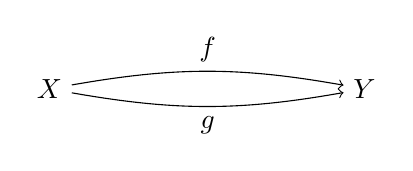
\begin{tikzpicture}
            \node (X) at (-2,0) {\(X\)};
            \node (Y) at (2,0) {\(Y\)};
            \draw[->] (X) to [bend left = 10] node[above] (f) {\(f\)} (Y);
            \draw[->] (X) to [bend right = 10] node[below] (g) {\(g\)} (Y);
        \end{tikzpicture}
    \end{center}
\end{definition}

\begin{lemma}
    \label {lemma:existence of limitation of homeomorphism}
    给出自然变换 \(\psi : \alpha \to \alpha^\prime\), 假使极限存在则存在唯一 \(\psi\) 使对任意 \(i\) 以下图表交换:

    \begin{center}
        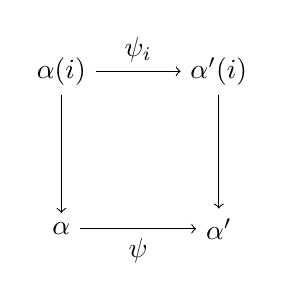
\begin{tikzpicture}
            \node (ai) at (-1,1) {\(\alpha (i)\)};
            \node (api) at (1,1) {\(\alpha^\prime (i)\)};
            \node (lima) at (-1,-1) {\(\varinjlim \alpha\)};
            \node (limap) at (1,-1) {\(\varinjlim \alpha^\prime\)};
            \draw[->] (ai) to node[above] (aii) {\(\psi_i\)} (api);
            \draw[->] (ai) to (lima);
            \draw[->] (api) to (limap);
            \draw[->] (lima) to node[below] (limf) {\(\varinjlim \psi\)} (limap);
        \end{tikzpicture}
    \end{center}

    \begin{proof}
        态射合成给出了 \(\alpha(i) \to \varinjlim \alpha^\prime\), 其与 \(\mathrm{Mor}(I)\) 相容, 由极限的定义唯一性给出了 \(\varinjlim \alpha \to \varinjlim \alpha^\prime\).
    \end{proof}
\end{lemma}

\begin{corollary}
    给出自然变换 \(\psi : \alpha \to \alpha^\prime\), 假使极限存在则存在唯一 \(\psi\) 使对任意 \(i\) 以下图表交换:

    \begin{center}
        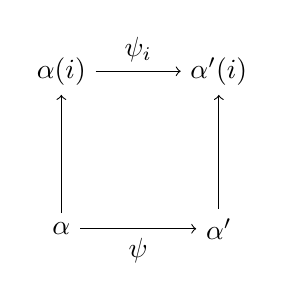
\begin{tikzpicture}
            \node (ai) at (-1,1) {\(\alpha (i)\)};
            \node (api) at (1,1) {\(\alpha^\prime (i)\)};
            \node (lima) at (-1,-1) {\(\varprojlim \alpha\)};
            \node (limap) at (1,-1) {\(\varprojlim \alpha^\prime\)};
            \draw[->] (ai) to node[above] (aii) {\(\psi_i\)} (api);
            \draw[->] (lima) to (ai);
            \draw[->] (limap) to (api);
            \draw[->] (lima) to node[below] (limf) {\(\varprojlim \psi\)} (limap);
        \end{tikzpicture}
    \end{center}
\end{corollary}

\begin{lemma}
    给出自然变换 \(\psi : \alpha_1 \to \alpha_2\),  \(\phi : \alpha_2 \to \alpha_3\), 假使极限存在则有等式 \(\varinjlim (\phi \psi) = \varinjlim \phi \varinjlim \psi\).

    \begin{proof}
            无非是交换图表:

            \begin{center}
                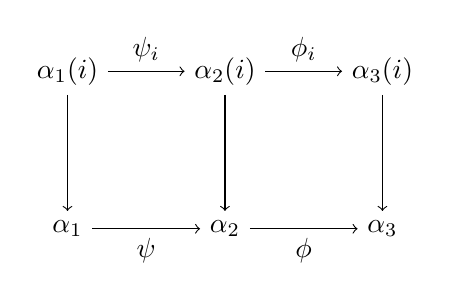
\begin{tikzpicture}
                    \node (a1i) at (-2,1) {\(\alpha_1 (i)\)};
                    \node (a2i) at (0,1) {\(\alpha_2 (i)\)};
                    \node (a3i) at (2,1) {\(\alpha_3 (i)\)};
                    \node (lima1) at (-2,-1) {\(\varinjlim \alpha_1\)};
                    \node (lima2) at (0,-1) {\(\varinjlim \alpha_2\)};
                    \node (lima3) at (2,-1) {\(\varinjlim \alpha_3\)};
                    \draw[->] (a1i) to node[above] (psi) {\(\psi_i\)} (a2i);
                    \draw[->] (a2i) to node[above] (phi) {\(\phi_i\)} (a3i);
                    \draw[->] (a1i) to (lima1);
                    \draw[->] (a2i) to (lima2);
                    \draw[->] (a3i) to (lima3);
                    \draw[->] (lima1) to node[below] (limpsi) {\(\varinjlim \psi\)} (lima2);
                    \draw[->] (lima2) to node[below] (limphi) {\(\varinjlim \phi\)} (lima3);
                \end{tikzpicture}
            \end{center}
    \end{proof}
\end{lemma}

\begin{corollary}
    同理有等式 \(\varprojlim (\phi \psi) = \varprojlim \phi \varprojlim \psi\).
\end{corollary}

\begin{lemma}
    直积的直积 (余积的余积) 为直积 (余积).

    \begin{proof}
        给出对象 \(X_{i,j}\) 的直积 \(X_{i} := \prod_j X_{i,j}\) 与直积 \(X := \prod_i X_i\),
        无非是说对于任意对象 \(Y\), \(\prod_{i,j} \mathrm{Hom} (Y,X_{i,j})\) 与 \(\prod_i \mathrm{Hom} (Y,X_i)\), \(\mathrm{Hom} (Y,X)\) 一一对应,
        老直积态射的合成给出新直积所需的态射.
    \end{proof}
\end{lemma}

\begin{definition}
    考察以下范畴 \(I\):

    \begin{center}
        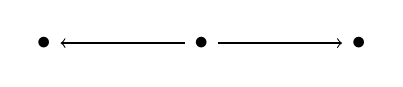
\begin{tikzpicture}
            \node (B1) at (-2,0) {\(\bullet\)};
            \node (B2) at (0,0) {\(\bullet\)};
            \node (B3) at (2,0) {\(\bullet\)};
            \draw[->] (B2) to (B1);
            \draw[->] (B2) to (B3);
        \end{tikzpicture}
    \end{center}

    以 \(I\) 为指标的极限称纤维积 (fibre product) 或拉回 (pullback), \(I\) 的余极限称纤维余积或推出 (pushout), 记作 Cartesius 图表:

    \begin{center}
        \begin{tikzpicture}
            \node (prod) at (-1,1) {\(X \times_Z Y\)};
            \node (X) at (1,1) {\(X\)};
            \node (Y) at (-1,-1) {\(Y\)};
            \node (Z) at (1,-1) {\(Z\)};
            \draw[->] (X) to (Z);
            \draw[->] (Y) to (Z);
            \draw[->] (prod) to (X);
            \draw[->] (prod) to (Y);
            \node at (0,0) {\(\Box\)};
        \end{tikzpicture} \begin{tikzpicture}
            \node (coprod) at (-1,1) {\(X \sqcup_Z Y\)};
            \node (X) at (1,1) {\(X\)};
            \node (Y) at (-1,-1) {\(Y\)};
            \node (Z) at (1,-1) {\(Z\)};
            \draw[->] (Z) to (X);
            \draw[->] (Z) to (Y);
            \draw[->] (X) to (coprod);
            \draw[->] (Y) to (coprod);
            \node at (0,0) {\(\boxplus\)};
        \end{tikzpicture}
    \end{center}
\end{definition}

\begin{definition}
    若范畴 \(\mathcal{C}\) 满足所有以某个小范畴为指标的 \(\varprojlim\) 存在
    则 \(\mathcal{C}\) 是完备的, 对称的 \(\varinjlim\) 存在则 \(\mathcal{C}\) 是余完备的.
\end{definition}

\begin{definition}
    定义拟序集 \(P\) 的范畴, 其对象为 \(P\) 中的元素, 在 \(X \leq Y\) 时 \(\abs{\mathrm{Hom} (X,Y)} = 1\) 的范畴.
\end{definition}

\begin{lemma}[Freyd]
    小范畴 \(\mathcal{C}\) 完备当且仅当 \(\mathcal{C}\) 从某个拟序集 \(P\) 构造出来, 且 \(P\) 中每个子集都有下确界.

    \begin{proof}
        假定有 \(f,g : X \to Y\), 则 \(\abs{\mathrm{Hom} (X,Y^{\abs{\mathrm{Mor} (\mathcal{C})}})} > \mathrm{Mor} (\mathcal{C})\)
        矛盾, 此时极限就是下确界.
    \end{proof}
\end{lemma}

\begin{theorem}
    假使范畴 \(\mathcal{C}\) 含所有直积与等化子, 则 \(\mathcal{C}\) 是完备的.

    \begin{proof}
        给出小范畴 \(I\) 与函子 \(F : I \to \mathcal{C}\), 令 \(X := \prod_{i \in \mathrm{Ob} (I)} F i\),
        \(Y := \prod_{\sigma \in \mathrm{Mor} (\mathcal{C})} F (t (\sigma))\), \(Z := \prod_{\sigma \in \mathrm{Mor} (\mathcal{C})} F (s (\sigma))\),
        考察 \(X \to Y\) 的两个态射, 一个逐点, 一个逐点透过 \(Z\), 然后透过 \(\sigma\), 其等化子自然与 \(\sigma\) 相容, 即为极限.
    \end{proof}
\end{theorem}

\begin{corollary}
    假使范畴 \(\mathcal{C}\) 含所有余积与余等化子, 则 \(\mathcal{C}\) 是余完备的.
\end{corollary}

\begin{lemma}
    \(\mathbf{Set}\) 是完备的.

    \begin{proof}
        显然 \(\mathbf{Set}\) 含所有直积, 余积, 等化子, 余等化子.
    \end{proof}
\end{lemma}

\begin{definition}[滤过]
    \setlabel {滤过}
    \label {definition:filtered category}
    给出小范畴 \(I\), 若任取 \(i,j \in \mathrm{Ob} (I)\), 存在 \(k \in \mathrm{Ob} (I)\), 使得 \(i,j\) 到 \(k\) 有态射,
    且对于任意 \(f,g : i \to j\), 存在 \(h : j \to k\), 使得 \(h f = h g\), 则称 \(I\) 滤过 (filtered).
\end{definition}

滤过的好处在于允许我们显式地在某些特定的范畴 (如 \(\mathbf(Set)\)) 中构造余极限, 因为此处等化子是可以直接写出来的等价关系.

\begin{lemma}
    \(\mathcal{C}^{\wedge}\) 与 \(\mathcal{C}^{\vee}\) 是完备且余完备的.

    \begin{proof}
        只需给 \(\mathcal{C}\) 中每一个点赋予极限与余极限, 利用 \ref {lemma:existence of limitation of homeomorphism} 即可.
    \end{proof}
\end{lemma}

这里要注意到嵌入的过程, 假若嵌入 \(\mathbf{Set}^\mathrm{op}\), 而在 \(\mathbf{Set}\) 中考虑对应极限, 需转换 \(\lim\) 方向.

\begin{lemma}
    函子 \(\alpha : I \to \mathcal{C}\) 余极限存在当且仅当米田嵌入之后的余极限可表, 极限亦然.

    \begin{proof}
        米田嵌入给出的 \(\mathrm{Hom}\) 集的对应无非就是极限的定义.
    \end{proof}
\end{lemma}

\begin{definition}
    极限存在时, 称函子 \(F\) 保 \(\varprojlim \alpha\), 如果 \(F \varprojlim \alpha \simeq \varprojlim F \alpha\), 亦定义保 \(\varinjlim \alpha\).
\end{definition}

\begin{corollary}
    取 \(X \in \mathcal{C}\), 则函子 \(\mathrm{Hom} (X,-)\) 保 \(\varprojlim\), \(\mathrm{Hom} (-,X)\) 保 \(\varinjlim\).
\end{corollary}

\begin{theorem}
    若 \(F \dashv G\), 则 \(F\) 保 \(\varinjlim\), \(G\) 保 \(\varprojlim\).

    \begin{proof}
        考察 \(\mathcal{C}^{\vee}\) 中的等式:

        \[
            \begin{aligned}
                \mathrm{Hom}_{\mathcal{D}} (F \varinjlim \alpha, -) & \simeq \mathrm{Hom}_\mathcal{C} (\varinjlim \alpha, G (-)) \\
                & \simeq \varinjlim \mathrm{Hom}_\mathcal{C} (\alpha (i), G (-)) \\
                & \simeq \varinjlim \mathrm{Hom}_\mathcal{D} (F \alpha (i), -) \\
                & \simeq \mathrm{Hom}_\mathcal{D} (\varinjlim F \alpha, -)
            \end{aligned}
        \]

        依米田嵌入全忠实性, 此给出二者之同构.
    \end{proof}
\end{theorem}
